\documentclass[a4paper]{llncs}

% \usepackage{latexsym}
%\usepackage{amsmath}
% \usepackage{xspace}

%\input prooftree

% to be removed in final version
\pagestyle{plain}

\title{Formal specification of Gemplus' electronic purse case study}

\author{
  Nestor Cata\~no Collazos
\and
  Marieke Huisman
}

\institute{
  INRIA Sophia-Antipolis, France \\ 
  \email{Nestor.Catano@sophia.inria.fr,
         Marieke.Huisman@sophia.inria.fr}
}


\newcommand{\comment}[1]{\marginpar{\framebox{\begin{minipage}{\marginparwidth}{#1}\end{minipage}}}}

\begin{document}
\input{texdefs.tex}

\maketitle


\begin{abstract}

\end{abstract}

\section{Introduction}
\label{SectIntro}
rien pour le moment





\section{General outline of the Electronic Purse}
\label{SectGenPurse}
All of the \textit{Smart Cards} applications are split out in two
parties$:$ an extern application to the card (called terminal) and an
internal one (called applet). The electronic purse is a
\textsc{JavaCard} application which intends to provide to card holder,
the ability to execute bank operations. This application is loaded in
the smart card as an applet. The figure~\ref{fig-cas-pur} shows the
general outline of \textit{the electronic purse}.




\begin{center}
\begin{figure}[hbt]
\rule{\linewidth}{0.3mm}
\\[2.5ex]
\centering
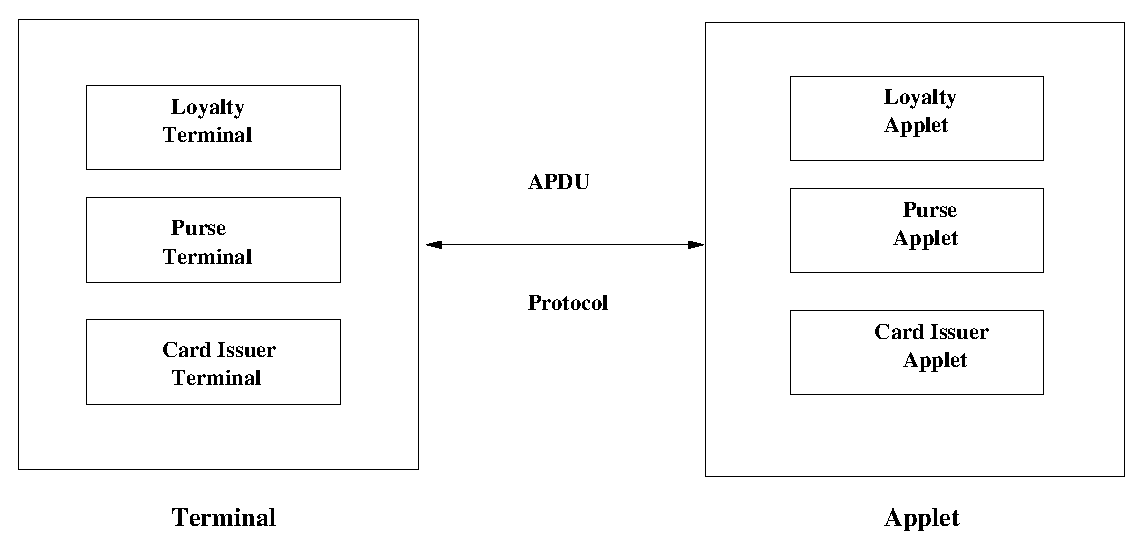
\epsfig{file=figures/javacard.eps, width=11cm, clip=}
\caption{Outline of the purse}
\label{fig-cas-pur}
\rule{\linewidth}{0.3mm}
\end{figure}
\end{center}




The  \texttt{CardIssuer} applet has personal information of the card
holder and contains the pine code of the card. The \texttt{Purse}
applet carries out the \textit{credit} and \textit{debit}
operations. This applet allows the card holder also to change its
currency type. Apart from that, this applet has several mechanisms
which do not allow to execute some commands when the applet is not
found in a suitable state. The applet \texttt{Loyalty} handle a
counter which is increased when any purchase done. When
a debit operation is failed, the application will see the available
money in this counter.


\paragraph{The \textit{debit} operation.}
This operation allow us to do a debit transaction. Thus, if
severals transaction are done in the same session, it is possible that 
the card user presents once his pine code for any transaction lesser than
\texttt{maxDebitWithOutPIN}. This variable represents the biggest
quantity that a client may credit without present his pine code. For
security reasons, the card holder can do at most
\texttt{maxTransactionWithoutPIN} transactions in a same session. 


\paragraph{The \textit{credit} operation.} When the purse is empty, the 
card holder can be do an debit operation. In this case, the terminal
sends the bank a request asking for any credit permission. If the card 
holder has some one the bank will send to the terminal a certificate of 
this permission. 



\paragraph{The \textit{Currency} operation.} The balance is related to a
currency. When the card holder travels he has the possibility to
change the currency. In this case, the terminal request to the bank a
new exchange rate and a certificate. The purse verifies than the bank is 
really the expected bank and it validates the exchange rate. After
changing the balance value, the purse must modify all the variables
that are related to the currency. \\

When a currency change occurs, the purse sends to the loyalties a
\textit{changeCurrency} warning. It is expected than each loyalty
requests to the purse all logged transaction.  Then the purse may erase 
the log transaction file. The purse can be associated to different
loyalties and it must differentiate them when the purse is sending
their logged transactions. \\






\section{Static checking of Java programs}
\label{SectStatic}


\subsection{\sc Esc/Java}
\label{SubSectEscJava}
\textsc{Esc/Java} is the verification tool developed at
Compaq SRC (Compaq Systems Research Center), which allow us to find
some errors in \textsc{Java} programs. \textsc{Esc/Java} allow us to
detect, at compile time, errors which usually are not detected until
run time. \\

\textsc{Esc/Java} includes an annotation langage with which
programmers can express design decisions using light weight
specifications. For example, one may give a method preconditions that
says than parameter is not null, or declare an object invariant that
says than an integer field lies between $0$ and the length of some
array field. \textsc{Esc/Java} uses the given annotations in reducing
spurious warnings, and also checks that the program is consistent with 
the given annotations. \\

\textsc{Esc/Java} performs a \textit{modular checking}, i.e,
\textsc{Esc/Java} checks each class separately. That means that
\textsc{Esc/Java} can be applied to code that calls libraries even if
the code for the libraries is not available. 






\section{Specification of the Electronic Purse}
\label{SectSpecPurse}






\subsection{The general specification approach}






\subsection{Interesting aspects of the specification}
The following sections present some interesting problems found in the
process of doing assertions for the purse application. These cases
highlight some commun programming problems and they show how an
verification tool can be used to find them. 



\subsubsection{Coding errors}
The \texttt{Decimal} class is a purse class and it allows us to
represent a floating point number as
composing by a decimal part and a integer part. These concepts are
represented by the variables \texttt{intPart} and \texttt{decPart}
respectively. This class is shown in the figure~\ref{fig-cla-dec}. The
method \texttt{isGreaterEqualThan} intends to decide when the decimal
represented by \texttt{this} is greater or equal than its parameter
\texttt{d}. Therefore, by mean of a \textsc{Esc/Java} assertion, we
have established a post-condition corresponding to this
specification. This work is done by an \texttt{ensures} comment, which
is shown on the line $8$. \\

After running the \textsc{Esc/Java} tool on this method, a warning
signal is activated. This warning suggest that this post-condition
will not be satisfied by the method. The problem is found on the line
$18$. This line must be replaced by \texttt{decPart >=
d.getDecPart()}. In this way, the condition asserted by the clause
\texttt{ensures} will be satisfied.


\begin{center}
\begin{figure}[hbt]
\rule{\linewidth}{0.3mm}
\rule{0em}{0.1ex}
\begin{tabbing}
pub\=lic\=cla\=ssD\=ecimale\=xtendsObject\kill
\emph{1.}\>$\mathtt{package com.gemplus.pacap.utils\ ;}$ \\
\\
\emph{2.}\>$\mathtt{public\ class\ {\bf Decimal}\ extends\ Object\{}$ \\
\>\>\vdots     \\
\emph{3.}\>\>{\it /*@ spec$\_$public */} $\mathtt{private\ short\ intPart\ =\
(short) 0\ ;}$ \\
\emph{4.}\>\>{\it /*@ spec$\_$public */} $\mathtt{private\ short\ decPart\ =\ (short)\ 0\ ;}$ \\
\>\>\vdots \\ 
\emph{5.}\>\>{\it /*@}  \\
\emph{6.}\>\>\>{\it //modifies $\backslash$nothing} \\
\emph{7.}\>\>\>{\it requires d $!=$ null;} \\
\emph{8.}\>\>\>{\it ensures $\backslash$ result $==$ (intPart $>$ d.intPart
$||$} \\
\emph{9.}\>\>\>\>{\it (intPart $==$
d.intPart $\&\&$ (decPart $==$ d.decPart $||$ decPart $>$ d.decPart))) ;} \\ 
\emph{10.}\>\>{\it */} \\
\emph{11.}\>\>$\mathtt{public\ boolean\ {\bf isGreaterEqualThan}(Decimal\ d)\{}$ \\
\emph{12.}\>\>\>$\mathtt{boolean\ resu\ =\ false\ ;}$ \\
\\
\emph{13.}\>\>\>$\mathtt{if(intPart\ >\ d.getIntPart())}$ \\
\emph{14.}\>\>\>\>$\mathtt{resu\ =\ true\ ;}$ \\
\emph{15.}\>\>\>$\mathtt{else\ if\ (intPart\ <\ d.getIntPart())}$ \\
\emph{16.}\>\>\>\>$\mathtt{resu\ =\ false\ ;}$ \\
\emph{17.}\>\>\>$\mathtt{else\ if(intPart\ ==\ d.getIntPart())\{} $        \\
\emph{18.}\>\>\>\>$\mathtt{if((decPart\ >\ d.getDecPart())\ ||\ (decPart\ >\
d.getDecPart()))}$ \\
\emph{19.}\>\>\>\>\>$\mathtt{resu\ =\ true\ ;}$ \\
\emph{20.}\>\>\>\>$\mathtt{else\ if\ (decPart\ <\ d.getDecPart())}$\\
\emph{21.}\>\>\>\>\>$\mathtt{resu = false;}$ \\
\emph{22.}\>\>\>$\mathtt{\}}$ \\
\emph{23.}\>\>\>$\mathtt{return\ resu\ ;}$ \\
\emph{24.}\>\>$\mathtt{\}}$ \\
\>\>\vdots \\
\emph{25.}\>$\mathtt{\}}$ 
\end{tabbing}
\caption{Piece of {\tt Decimal} class}
\label{fig-cla-dec}
\rule{\linewidth}{0.3mm}
\end{figure}
\end{center}




\subsubsection{Final modifiers}
The \texttt{Annee} class allows to represent a \textit{year} in the
\texttt{purse} application. The Figure~\ref{fig-cla-ann} presents its
source code with \textsc{Esc/Java}assertions. This class declares two 
static variables called \texttt{MIN} and \texttt{MAX}, which represent
the minimum and maximum year allowed by the application
respectively. This class declares
also an invariant which relates these values. The static method
\texttt{check} allow us to verify that its parameter is a valid
year. \\

The figure~\ref{fig-cla-dat} shows the \texttt{Date} class. This class
represents a date for the application$:$ \texttt{jour}(day),
\texttt{mois}(month), \texttt{annee}(year). We have established some
invariants for this class, which allow the purse application to place
each of them between valide intervals. The method \texttt{setDate}
assigns some values to the internal variables as long as
these variables have valide values, i.e, these variables verify the
conditions expressed by the clauses ensures. In this way, if the
pre-condition is satisfied, the internal variables will be assigned
with the values of their parameters. Otherwise, the method will raise
an \texttt{DateException} exception. This abnormality condition is
declared by the \texttt{exsures} clause. \\

\textsc{Esc/Java} complains when it finds a declaration such as$:$ \\
\mbox{\tt date.setDate((byte)1, (byte)1, (byte)110);} (where date is a
\texttt{Date} instance). The warning message signals that its third
parameter does not verify the condition established by the clause
\texttt{requires} belonging to the method \texttt{setDate} (line
$5$). This warning is desployed in spite of this call respect the
requires condition, i.e, $110>=99\ \&\&\ 110<= 127$. \\

The problem is happend due to the wrong declaration of \textsc{MIN}
and \textsc{MAX} variables belonging to the \texttt{Annee}
class. These variables were not declared as \texttt{final}~\footnote{{\sc
Java} does not allow to change in runtime the value of a final {\tt
final} variable.}. Thus, their values could be changed in runtime by
mean of a direct assignation~\footnote{In fact, due to these variables
are declared are \texttt{public}} and the pre-condition would be not
satisfied. \\


The declaration variables as \texttt{static} (commun for all instance)
and \texttt{final} (which can not be changed) prevent us of doing
any assumption that will be not satisfied any more by an
application. This kind of control is carried out by
\textsc{Esc/Java}. \\


\begin{center}
\begin{figure}[htb]
\rule{\linewidth}{0.3mm}
\\[2.0ex]
\begin{tabbing}
pub\=lic\=cla\=ssD\=ate  \kill
$\mathtt{package\ com.gemplus.pacap.utils\ ;}$ \\
 \\
$\mathtt{public\ abstract\ class\ {\bf Annee}\ extends\ Object\ \{}$ \\
\>{\it //@ invariant MIN $<=$ MAX} \\
 \\ 
\>$\mathtt{public\ static\ byte\ MIN\ =\ (byte)99\ ;} $\\
\>$\mathtt{public\ static\ byte\ MAX\ =\ (byte)127\ ;} $\\
\\
\\
\>{\it /*@} \\
\>\>{\it //modifies $\backslash$nothing ;} \\
\>\>{\it requires true ;} \\
\>\>{\it ensures $\backslash$result $==$ (j $>=$ MIN $\&\&$ j $<=$ MAX) ;} \\
\>\>{\it //exsures (RuntimeException)false ;} \\
\>*/ \\
\>$\mathtt{public\ static\ boolean\ {\bf check}(byte\ j)\ \{} $ \\
\>\>$\mathtt{return\ ((j\ >=\ Annee.MIN)\ \&\&\ (j\ <=\ Annee.MAX))\ ;}$  \\
\>$\mathtt{\}} $ \\
$\mathtt{\}} $ \\
\end{tabbing}
\caption{{\tt Annee} class}
\label{fig-cla-ann}
\rule{\linewidth}{0.3mm}
\end{figure}
\end{center}





\begin{center}
\begin{figure}[hbt]
\rule{\linewidth}{0.3mm}
\\[2.0ex]
\begin{tabbing}
pub\=lic\=cla\=ssD\=ate\=ext\=endsObject  \kill
$\mathtt{public\ class\ {\bf Date}\ extends\ Object\ \{}$ \\

\>{\it /*@} \\
\>\>{\it invariant jour $>=$ Jour.MIN $\&\&$ jour $<=$ Jour.MAX ;} \\	
\>\>{\it invariant mois $>=$ Mois.MIN $\&\&$ mois $<=$ Mois.MAX ;} \\
\>\>{\it invariant annee $>=$ Annee.MIN $\&\&$ annee $<=$ Annee.MAX ;} \\
\>{\it */}
\\
\\
\>{\it /*@ spec$\_$public */} $\mathtt{private\ byte\ jour\ =\ Jour.MIN\ ;}$ \\
\>{\it /*@ spec$\_$public */} $\mathtt{private\ byte\ mois\ =\ Mois.MIN\ ; }$ \\   
\>{\it /*@ spec$\_$public */} $\mathtt{private\ byte\ annee\ =\ Annee.MIN\ ;}$ \\
\\ 
\\
\emph{1. }\>{\it /*@} \\ 
\emph{2. }\>\>{\it modifies jour, mois, annee ;} \\
\emph{3. }\>\>{\it requires j $>=$ Jour.MIN  $\&\&$ j $<=$ Jour.MAX ;} \\
\emph{4. }\>\>{\it requires m $>=$ Mois.MIN  $\&\&$ m $<=$ Mois.MAX ;} \\
\emph{5. }\>\>{\it requires a $>=$ Annee.MIN $\&\&$ a $<=$ Annee.MAX ;} \\
\emph{6. }\>\>{\it ensures jour $==$ j $\&\&$ annee $==$ a $\&\&$ mois $==$ m ;} \\
\emph{7. }\>\>{\it exsures (DateException) false ;} \\
\emph{8. }\>{\it */} \\
\>$\mathtt{public\ void\ {\bf setDate}(byte\ j,\ byte\ m,\ byte\ a)\ throws\ DateException\{}$ \\
\>\>{\it // check the day } \\        
\>\>$\mathtt{if(!Jour.check(j)) \{}$ \\
\>\>\>$\mathtt{DateException.throwIt(DateException.ERREUR\_JOUR)\ ;}$ \\
\>\>$\mathtt{\}else\ \{}$ \\
\>\>\>{\it // check the month} \\
\>\>\>$\mathtt{if(!Mois.check(m))\ \{}$\\
\>\>\>\>$\mathtt{DateException.throwIt(DateException.ERREUR\_MOIS)\ ;}$ \\
\>\>\>$\mathtt{\}else\ \{}$ \\
\>\>\>\>{\it // check the year} \\
\>\>\>\>$\mathtt{if(!Annee.check(a)) \{}$ \\
\>\>\>\>\>$\mathtt{DateException.throwIt(DateException.ERREUR\_ANNEE)\ ;}$ \\
\>\>\>\>$\mathtt{\}else\ \{}$ \\
\>\>\>\>\>{\it $\slash \slash$ all is good} \\
\>\>\>\>\>$\mathtt{jour\ =\ j\ ;} $\\
\>\>\>\>\>$\mathtt{mois\ =\ m\ ;} $\\
\>\>\>\>\>$\mathtt{annee\ =\ a\ ;} $\\
\>\>\>\>$\mathtt{\}}$ \\
\>\>\>$\mathtt{\}} $\\
\>\>$\mathtt{\}} $\\
\>$\mathtt{\}} $\\
\>$\vdots$ \\
$\mathtt{\}}$ \\
\end{tabbing}
\caption{{\tt Date} class}
\label{fig-cla-dat}
\rule{\linewidth}{0.3mm}
\end{figure}
\end{center}






\subsubsection{Implicit invariants}
The figure~\ref{fig-cla-acc} shows the \texttt{AccessCondition}
class. This class models the access conditions for the purse
commands. These access conditions are represented by the variables
\texttt{FREE}, \texttt{LOCKED}, \texttt{SECRET$\_$CODE} and
\texttt{SECURE$\_$MESSAGING}. The internal variable \texttt{condition} 
may take one of these values. According to the purse
specification~\cite{BMGL00}, the \texttt{AccessCondition} class have
to verify the following invariant$:$ \\

\begin{tabbing}
//@ invariant \=condition == FREE || condition == LOCKED \kill
{\it $\slash\slash$@ invariant condition $==$ FREE $||$} \\
\>{\it condition $==$ LOCKED $||$} \\
\>{\it condition $==$ SECRET$\_$CODE $||$} \\
\>{\it condition $==$ SECURE$\_$MESSAGING $||$} \\
\>{\it condition $==$ (SECURE$\_$MESSAGING $|$ SECRET$\_$CODE)} \\
\end{tabbing}

This invariant establishes that the variable \texttt{condition} only
takes a value declared in this class. This invariant is rejected by
the \textsc{Esc/Java} compiler. The problem is found on the line
$15$. There, its constructor initialises the variable
\texttt{condition} to a value which have not been considered by the
class \texttt{AccessCondition}. Apart from that, strangely this
variable have been initialised to $FREE$ on the line $7$ and to $0$
in the class constructor.




\begin{center}
\begin{figure}[hbt]
\rule{\linewidth}{0.3mm}
\rule{0em}{0.1ex}
\begin{tabbing} 
pac\=kag\=eco\=m.gemplus.pacap.purse; \kill 
\emph{1.}\>$\mathtt{package com.gemplus.pacap.purse;}$\\
\\
\emph{2.}\>$\mathtt{public\ class\ {\bf AccessCondition}\ extends\ Object\{}$\\

\emph{3.}\>\>$\mathtt{public\ static\ final\ byte\ FREE\		=\ (byte)1\ ;}$\\
\emph{4.}\>\>$\mathtt{public\ static\ final\ byte\ LOCKED\		=\ (byte)2\ ;}$\\
\emph{5.}\>\>$\mathtt{public\ static\ final\ byte\ SECRET\_CODE\	=\ (byte)4\ ;}$\\
\emph{6.}\>\>$\mathtt{public\ static\ final\ byte\ SECURE\_MESSAGING\	=\
(byte)8\ ; }$\\
\\
\emph{7.}\>\>{\it /*@ spec$\_$public */} $\mathtt{private\ byte\ condition\ =\ FREE\ ;}$\\
\\
\emph{8.}\>\>{\it /*@ }\\
\emph{9.}\>\>\>{\it requires true ;}\\
\emph{10.}\>\>\>{\it ensures condition $==$ (byte)0 ;}\\
\emph{11.}\>\>\>{\it ensures $\backslash$fresh(this) ;}\\
\emph{12.}\>\>{\it */} \\
\emph{13.}\>\>$\mathtt{public\ {\bf AccessCondition}(\ ) \{}$\\
\emph{14.}\>\>\>$\mathtt{super()\ ;}$\\
\emph{15.}\>\>\>$\mathtt{setCondition((byte)0)\ ;}$\\
\emph{16.}\>\>$\mathtt{\}}$\\

\>\>\vdots \\

\emph{17.}\>\>{\it /*@ } \\
\emph{18.}\>\>\>{\it modifies condition ;} \\
\emph{19.}\>\>\>{\it requires true ;} \\
\emph{20.}\>\>\>{\it ensures condition $==$ c ;} \\
\emph{21.}\>\>{\it */} \\
\emph{22.}\>\>$\mathtt{public\ void\ {\bf setCondition}\ (byte\ c)\{}$\\
\emph{23.}\>\>\>$\mathtt{condition\ =\ c\ ;}$\\
\emph{24.}\>\>$\mathtt{\}}$\\

\>\>\vdots \\
\emph{25.}\>$\mathtt{\}}$
\end{tabbing}
\caption{Piece of {\tt AccessCondition} class}
\label{fig-cla-acc}
\rule{\linewidth}{0.3mm}
\end{figure}
\end{center}




\subsubsection{Unnecessary try-catches}




\subsubsection{``Ugly'' modifications}




\subsection{The corrected version of the Electronic Purse}






\section{Conclusions}
\label{SectConcl}

\end{document}


